\documentclass[12pt]{article}
\usepackage[utf8]{inputenc}
\usepackage{amsmath} 
\usepackage{multicol} 
\usepackage{graphicx} 
\usepackage{float} 
\usepackage[sorting=none]{biblatex}
\bibliography{bibs.bib}
\usepackage{dsfont} 
\usepackage{textcomp} 
\usepackage{multirow} 
\usepackage{amsfonts} 
\usepackage[colorlinks=True]{hyperref}
\hypersetup{linkcolor=black,
citecolor=blue}
\usepackage{cleveref} 
\usepackage{fancyhdr} 
\setlength{\headheight}{14.5pt} 
\renewcommand{\sectionmark}[1]{\markright{#1}{}} 
\usepackage[T1]{fontenc} 
\usepackage[colorinlistoftodos]{todonotes} 
\usepackage[margin=2cm,a4paper]{geometry} 
\newgeometry{left=2.0cm,right=2.0cm,top=2.5cm,bottom=2.0cm} 
\usepackage{listings}
\setlength{\marginparwidth}{2cm} 
\usepackage[onehalfspacing]{setspace}
\setlength{\parindent}{0pt} 
\newcommand{\deriv}{\mathrm{d}} 
\title{} 
\pagestyle{fancy} 
\fancyhf{} 
\rhead{\leftmark} 
\lhead{Very Near Sun Exploration} 
\rfoot{Page \thepage} 
\renewcommand{\headrulewidth}{1pt} 
\renewcommand{\footrulewidth}{1pt} 
\begin{document}
\begin{titlepage}
\newgeometry{left=1.0in,right=1.0in,top=2.0in,bottom=1.0in}
\newcommand{\HRule}{\rule{\linewidth}{0.5mm}}
\begin{centering} 
%---------------------------------------------------------------------------
%	HEADING SECTIONS
%---------------------------------------------------------------------------

\includegraphics[scale=0.6]{Media/Document/Uni_of_Kent.png}\\
%---------------------------------------------------------------------------
%	TITLE SECTION
%---------------------------------------------------------------------------
\vspace{1.0cm} 
\large{\emph{Division of Natural Sciences, University of Kent in Canterbury}} \\ [0.1cm]
\large{Department of Physical Sciences, Ingram Building} \\ [1.0cm]
\Huge{\bfseries{Magnox Radioactive Waste \\ Disposal Container}} \\ [1.0cm]
{\Large \bfseries{By \\ [0.2cm] Lukasz R Tomaszewski}}\\[0.2cm]
\textsc{\large BSc (Hons) Astronomy, Space Science and Astrophysics}\\ [-0.2cm]
\textsc{\large PH617: Physics Project Laboratory}\\ [-0.2cm]
\textsc{\large Word Count: 6260 (LaTeX)}\\ [1.5cm]
{\Large \bfseries{March 2021}}\\
\end{centering} 
\end{titlepage}
%---------------------------------------------------------------------------
\newpage
\begin{titlepage}
\begin{tableofcontents}
\end{tableofcontents}
\end{titlepage}
\newpage
%--------------------------------------------------------------------------------

\section{Assignment Brief}
\label{Assignment Brief Section}

The assessment is based upon the Emergent explorations to be found in "Computational Explorations in Cognitive Neuroscience". Note that you have covered some of these explorations in the practical classes. \\

\emph{Can you submit your assignment as a pdf document? If you write anything by hand, e.g. maths derivations, can you include that as an image, preferably in the same document as the rest of your assessment.} 

\section{Exploration Questions}
\label{Exploration Questions Section}
\subsection{Q1: Exploration 2.6.1 (Page 49)}
\label{Q1:Expl 2.6.1 SubSection}

\subsubsection{Task 2.1}
\label{Q1:Expl 2.6.1(2.1) SubSubSection}

\begin{tcolorbox}[colback=gray!20!white,colframe=gray!20!white]
  \emph{\textbf{Question 2.1 (a)} Describe the effects on the neural response of increasing $g_{bar\_e}$ to .5, and of decreasing it to .3. \textbf{(b)} Is there a qualitative difference in the unit activation (act) between these two changes of magnitude .1 away from the initial .4 value? \textbf{(c)} What important aspect of the point neuron activation function does this reveal? [Mark: 11]} 
\end{tcolorbox} 
\vspace{0.5cm}

When increasing the value of the excitatory conductance ($g_{bar\_e}$) from 0.4 to 0.5, the value of the activation value for a neural response (receiving unit) increases from 0.7204 to 0.9445 as showing in \cref{Q2.1 - 0.4} and \cref{Q2.1 - 0.5} and indicating a relationship between the excitatory conductance ($g_{bar\_e}$) and the receiving unit. When changing $g_{bar\_e}$ from 0.4/0.5 to 0.3, the neural response is null as seen in \cref{Q2.1 - 0.3}, where the receiving unit doesn't pick up any value despite the sending unit ($g_{bar\_i}$) remaining the same. When comparing the graphical output data shown in \cref{Q2.1 - 0.4G}, \cref{Q2.1 - 0.5G} and \cref{Q2.1 - 0.3G} for the 3 values of $g_{bar\_e}$ (0.4, 0.5 and 0.3 respectively). The activation value stems from the membrane potential ($V_m$), which for all 3 graphs shows a 0.2241 increase for $g_{bar\_e}$ at 0.4 to 0.5, Ultimately when $g_{bar\_e}$ equals 0.3 then the activation value flat lines in \cref{Q2.1 - 0.3G} as it return a null value. This highlights how the point neuron activation function relates to the input excitatory conductance directly affects the total activation value.

\newpage
\begin{multicols}{2}
\begin{figure}[H]
\centering
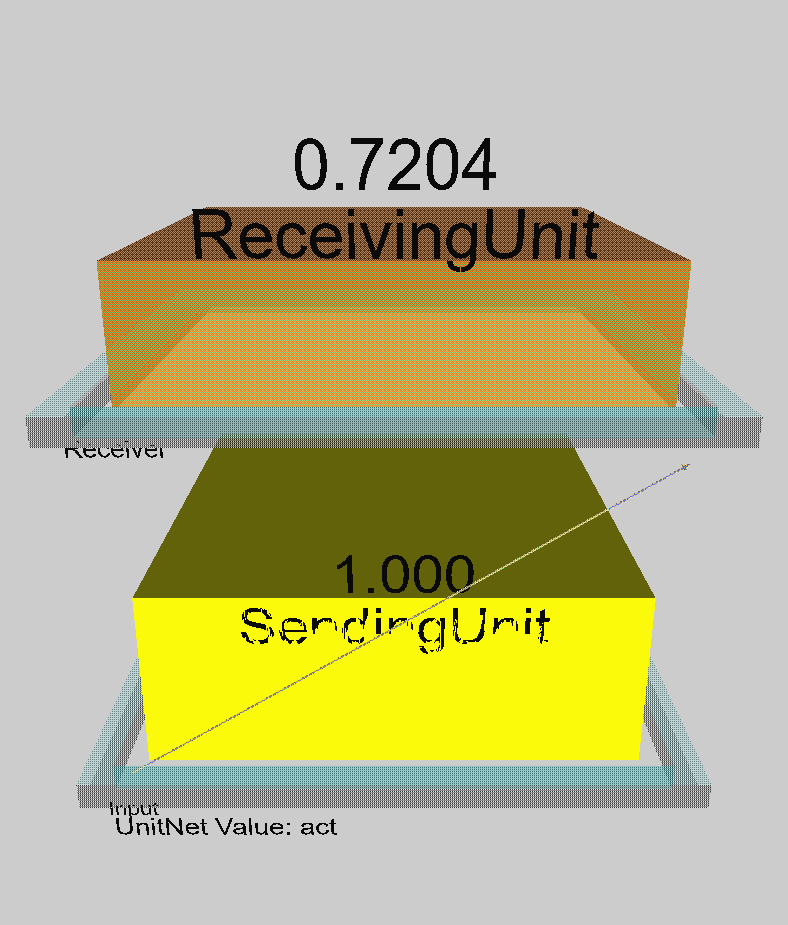
\includegraphics[scale=0.225]{Media/Main/EQ1/2.1.A.png}
\caption{Visual representation of the sending and receiving units with $g_{bar\_e}$.}
\label{Q2.1 - 0.4}
\end{figure}

\begin{figure}[H]
\centering
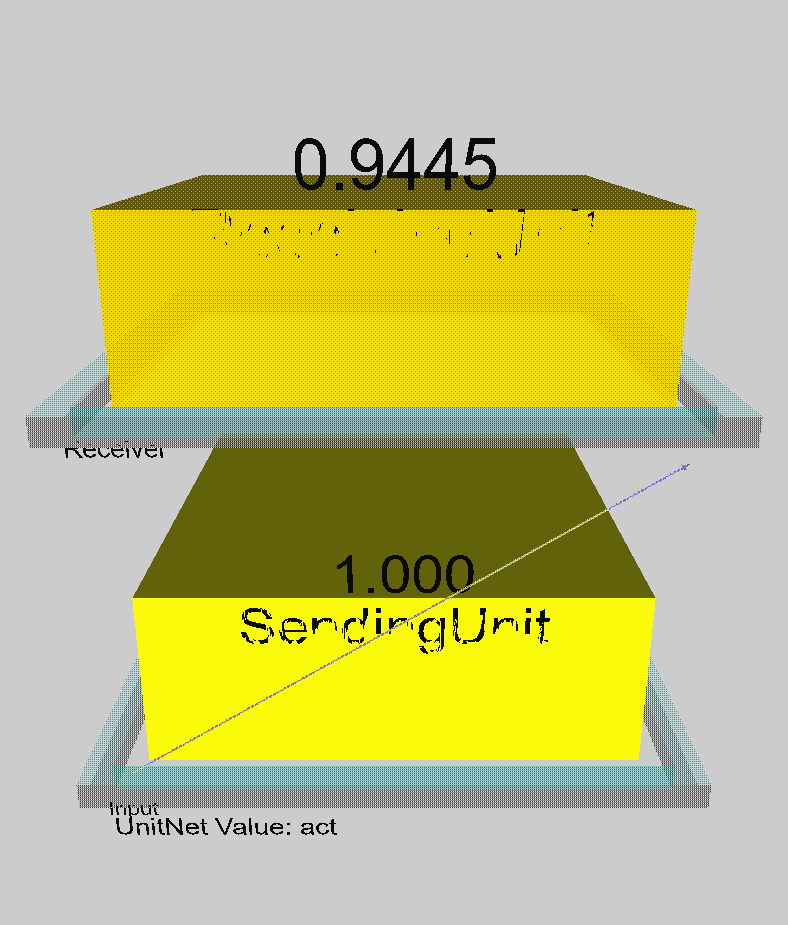
\includegraphics[scale=0.225]{Media/Main/EQ1/2.1.Aa.png}
\caption{Visual representation of the sending and receiving units with $g_{bar\_e}$.}
\label{Q2.1 - 0.5}
\end{figure}

\begin{figure}[H]
\centering
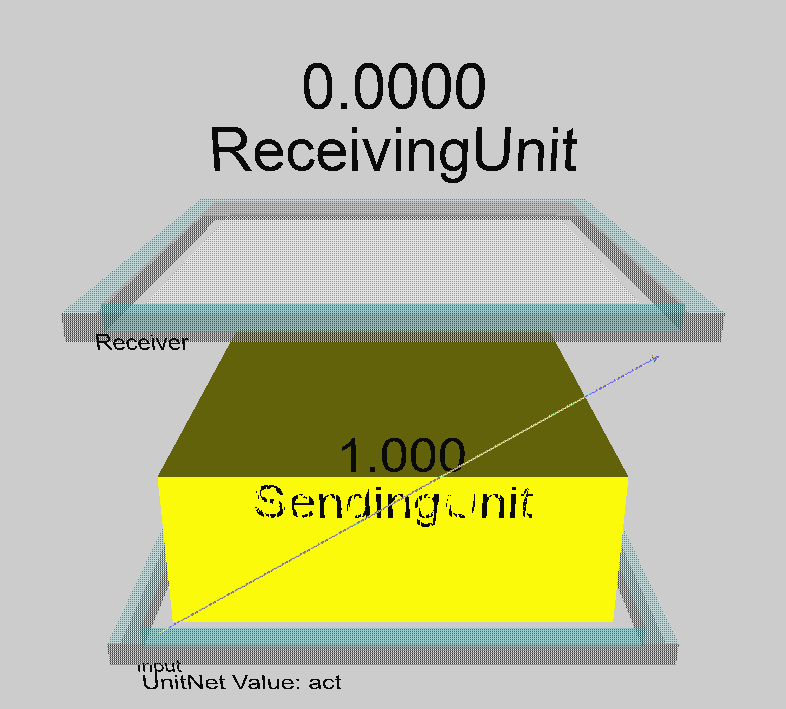
\includegraphics[scale=0.225]{Media/Main/EQ1/2.1.Ab.png}
\caption{Visual representation of the sending and receiving units with $g_{bar\_e}$.}
\label{Q2.1 - 0.3}
\end{figure}

\begin{figure}[H]
\centering
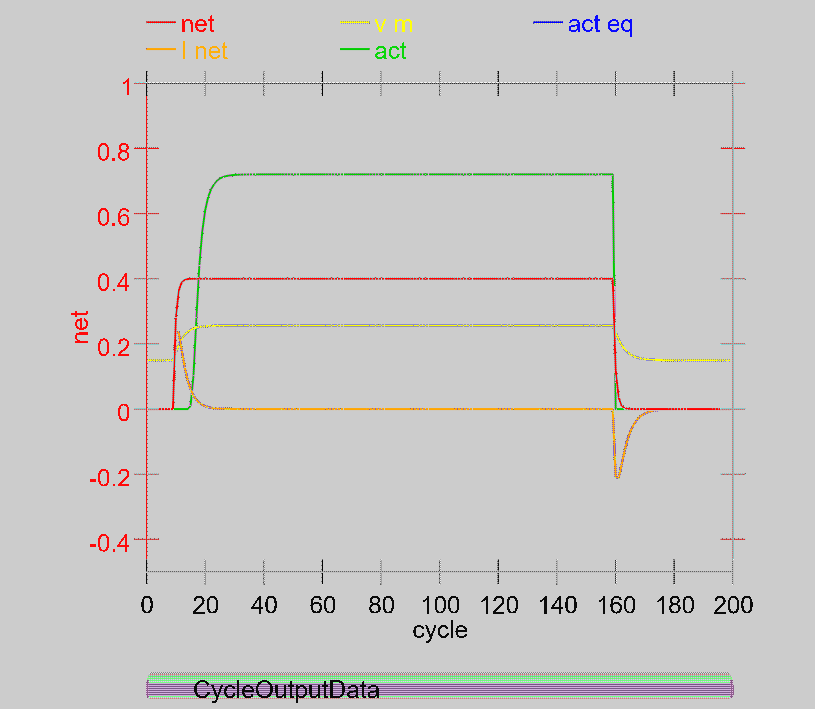
\includegraphics[scale=0.3]{Media/Main/EQ1/2.1.AG.png}
\caption{Graphical output data of \cref{Q2.1 - 0.4} when running a value of 0.4 for $g_{bar\_e}$.}
\label{Q2.1 - 0.4G}
\end{figure}

\begin{figure}[H]
\centering
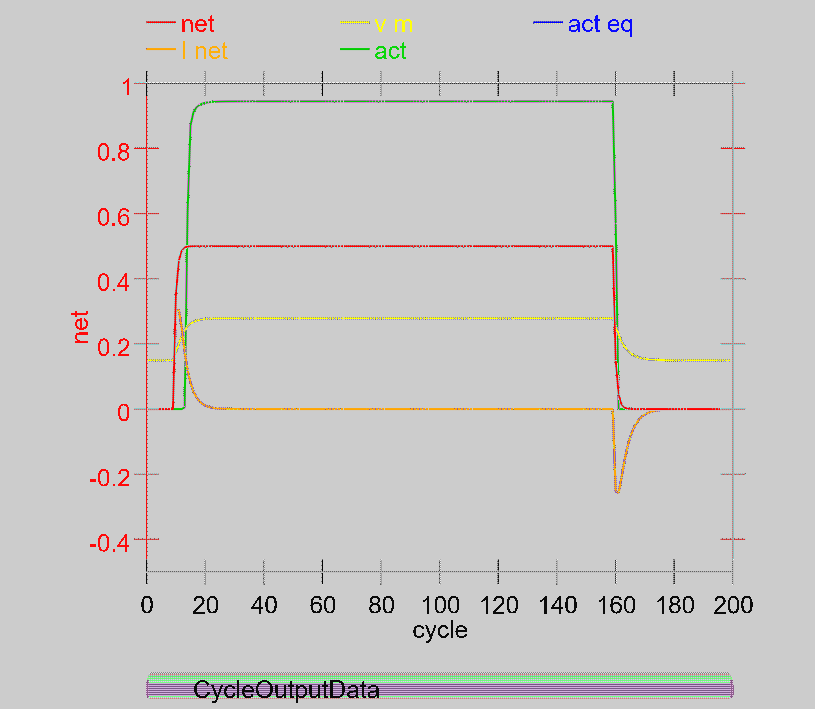
\includegraphics[scale=0.3]{Media/Main/EQ1/2.1.AaG.png}
\caption{Graphical output data of \cref{Q2.1 - 0.5} when running a value of 0.5 for $g_{bar\_e}$.}
\label{Q2.1 - 0.5G}
\end{figure}

\begin{figure}[H]
\centering
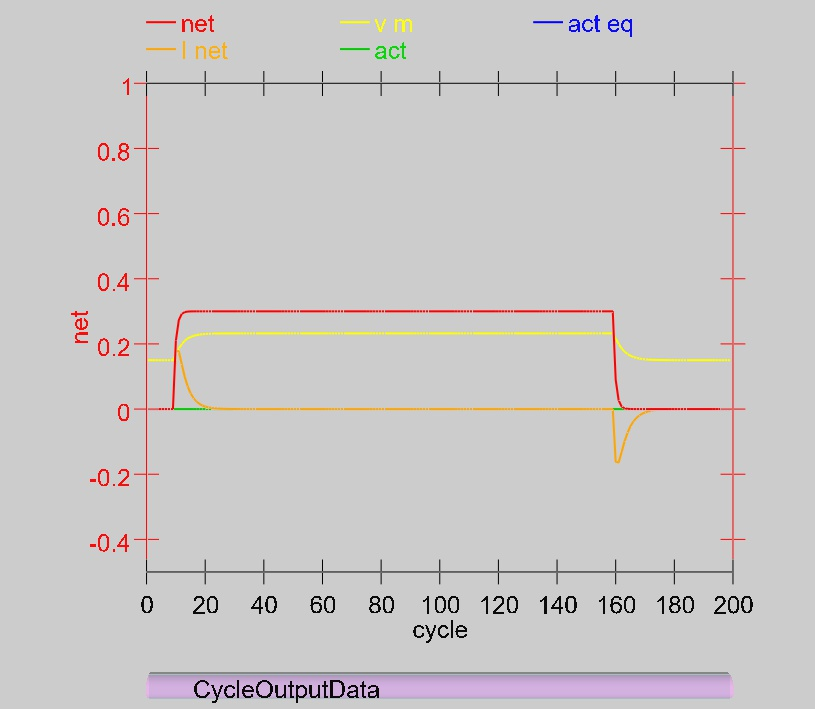
\includegraphics[scale=0.3]{Media/Main/EQ1/2.1.AbG.png}
\caption{Graphical output data of \cref{Q2.1 - 0.3} when running a value of 0.3 for $g_{bar\_e}$.}
\label{Q2.1 - 0.3G}
\end{figure}
\end{multicols}


\subsubsection{Task 2.2}
\label{Q1:Expl 2.6.1(2.2) SubSubSection}

\begin{tcolorbox}[colback=gray!20!white,colframe=gray!20!white]
  \emph{\textbf{Question 2.2 (a)} To 3 decimal places, what value of $g_{bar\_e}$ puts the unit just over threshold? Can you think of a better way of finding this value (Hint: Do you remember an equation for the equilibrium membrane potential given a particular set of inputs?) \textbf{(b)} Compute the exact value of excitatory input required to just reach threshold, showing your math (note that: $g_l$ is always 1 because the leak channels are always open; $g_e$ is 1 when the input is on; inhibition is not present here and can be ignored). Does this agree with your empirically determined value? \textbf{(Hint: It should!)} [Mark: 8]}
\end{tcolorbox} 
\vspace{0.5cm}

By experimenting with different values for $g_{bar\_e}$ less than 0.4 to determine the threshold of the receiving unit where its value is limited to 0.0001 at a minimum $g_{bar\_e}$ value of 0.324 (restricted to 3 decimal places). By using the equilibrium membrane potential equation, the minimum value of $g_{bar\_e}$ can be calculated to which reaches threshold of the neural response. \\

\textbf{Equilibrium Membrane Potential Equation:}
\begin{equation}
0 = g_e(t) \bar{g_e} (E_e - V_m(t))+ g_i(t) \bar{g_i} (E_i - V_m(t)) + g_l(t) \bar{g_l} (E_l - V_m(t))
\label{Equil Memb Pot Eq}
\end{equation}

\textbf{Re-Written As:}
\begin{equation}
V_m = \dfrac{g_e \bar{g_e}}{g_e \bar{g_e} + g_i \bar{g_i} + g_l \bar{g_l}} E_e + \dfrac{g_e \bar{g_e}}{g_e \bar{g_e} + g_i \bar{g_i} + g_l \bar{g_l}} E_i + \dfrac{g_e \bar{g_e}}{g_e \bar{g_e} + g_i \bar{g_i} + g_l \bar{g_l}} E_l
\label{New Equil Memb Pot Eq}
\end{equation}

\textbf{Alternative Formulation:}
\begin{equation}
V_m = \dfrac{g_e \bar{g_e} E_e + g_i \bar{g_i} E_i + 1 \bar{g_l} E_l}{g_e \bar{g_e} + g_i \bar{g_i} + g_l \bar{g_l}}
\label{Alt Equil Memb Pot Eq}
\end{equation}

\textbf{Excitatory Input Calculation:}
\begin{equation}
V_m = \dfrac{g_e \bar{g_e} E_e + g_l \bar{g_l} E_l}{g_e \bar{g_e} + g_l \bar{g_l}} \rightarrow \dfrac{g_e \bar{g_e} E_e + 1 \bar{1} E_l}{g_e \bar{g_e} + 1 \bar{1}} \rightarrow \dfrac{g_e \bar{g_e} E_e + E_l}{g_e \bar{g_e} + 1} 
\label{Q2.2 Calculation}
\end{equation}

\begin{equation}
\dfrac{g_e \bar{g_e} E_e}{g_e \bar{g_e}} = V_m - \dfrac{E_l}{1} \rightarrow V_m - E_l
\label{Q2.21 Calculation}
\end{equation}

\begin{equation}
E_e = V_m - E_l
\label{Q2.22 Calculation}
\end{equation}

\subsubsection{Task 2.3}
\label{Q1:Expl 2.6.1(2.3) SubSubSection}

\begin{tcolorbox}[colback=gray!20!white,colframe=gray!20!white]
  \emph{\textbf{Question 2.3 (a)} How does the response of the unit change when you change $g_{bar\_l}$? Why? \textbf{(b)} How does this differ from changes to $g_{bar\_e}$? \textbf{(c)} Use the same technique you used in the previous question to compute the exact amount of leak current necessary to put the membrane potential exactly at threshold when the $g_{bar\_e}$ value is at the default of .4 (show your math). [Mark: 11]}
\end{tcolorbox} 
\vspace{0.5cm}

The original input values are graphical plotted in \cref{Q2.30} to provide a reference when changing the value of $g_{bar\_l}$. The reference value of $g_{bar\_l}$ is 2.8, where all other variables are set in \cref{Q2.3 Table} and the comparing all the graphical plots, it's clear to see that the activation value of the receiving unit increasing when the original value of $g_{bar\_l}$ is decreased, then vice versa where the activation value decreases when $g_{bar\_l}$ is increased. When changing $g_{bar\_e}$, the net input is changed whereas the activation value changes as well, where when increasing $g_{bar\_e}$, the activation value increases as well and as it decreases, the activation value decreases also. However in the case of $g_{bar\_l}$ as it increases the value of the activation value decreases, the opposite of what happens with $g_{bar\_e}$. \\ 


\begin{table}[H]
\begin{center}
 \footnotesize
 \begin{tabular}{|c||c|c|c|c|c||c|}
 \hline
 \multicolumn{7}{|c|} {} \\
  States & $g_{bar\_e}$ & $g_{bar\_l}$ & $g_{bar\_i}$ & $g_{bar\_h}$ & $g_{bar\_a}$ & Graphical Plot\\
 \hline \hline
 0 & 0.4 & 2.8 & 1.0 & 0.1 & 0.1 & \cref{Q2.30}\\\hline
 1 & 0.4 & 3.0 & 1.0 & 0.1 & 0.1 & \cref{Q2.31} \\\hline
 2 & 0.4 & 3.2 & 1.0 & 0.1 & 0.1 & \cref{Q2.32} \\\hline
 3 & 0.4 & 2.5 & 1.0 & 0.1 & 0.1 & \cref{Q2.33} \\\hline
 4 & 0.4 & 2.2 & 1.0 & 0.1 & 0.1 & \cref{Q2.34} \\\hline
 \end{tabular} \\ 
 \caption{Tabulated results of changing $g_{bar\_l}$.}
 \label{Q2.3 Table}
\end{center}
\end{table}


\begin{figure}[H]
\centering
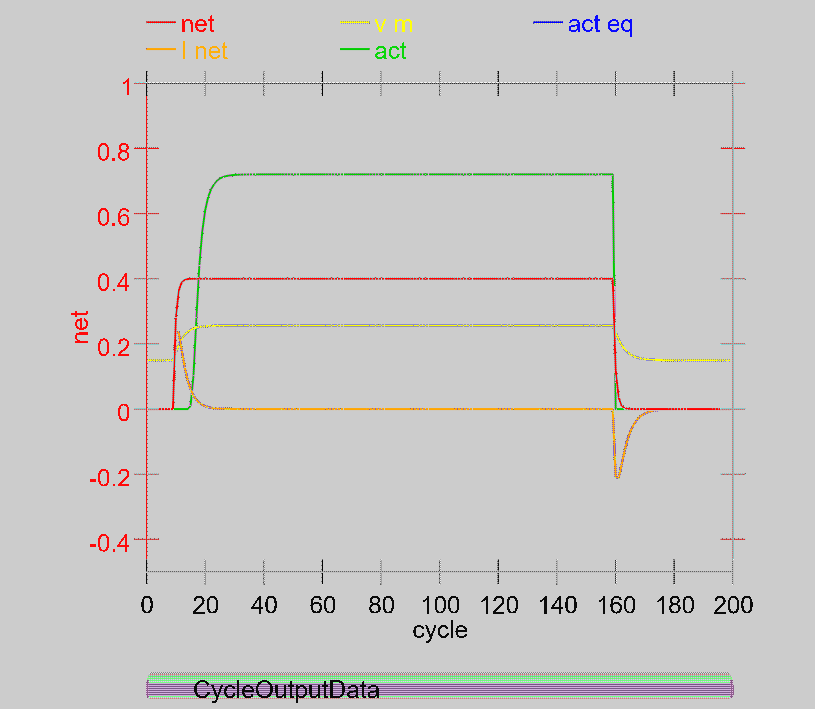
\includegraphics[scale=0.5]{Media/Main/EQ1/2.1.AG.png}
\caption{Graphical output of the system where $g_{bar\_l}$ is at the original value of 2.8.}
\label{Q2.30}
\end{figure}

\newpage

\begin{multicols}{2}
\begin{figure}[H]
\centering
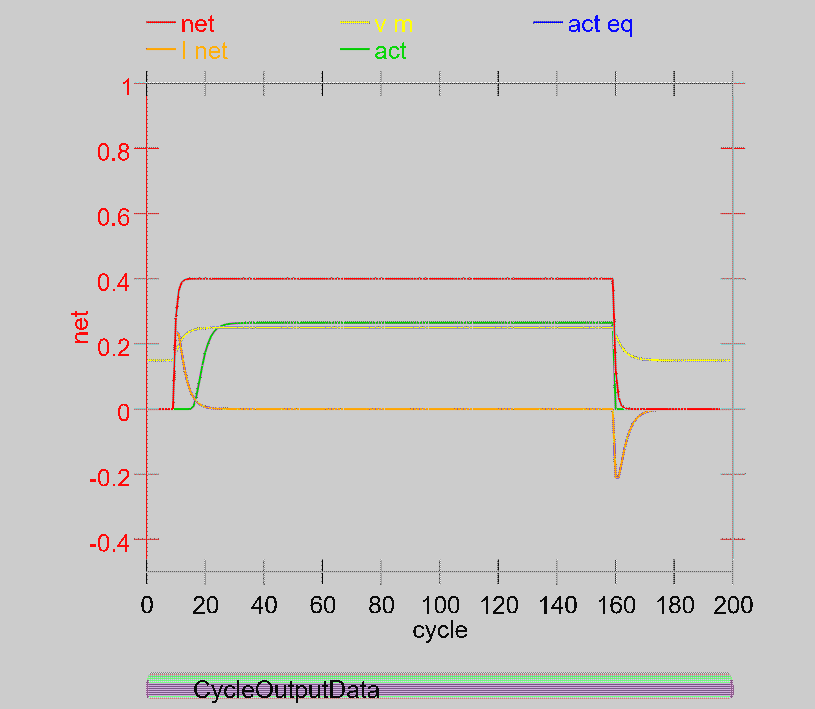
\includegraphics[scale=0.4]{Media/Main/EQ1/2.3.S1G.png}
\caption{Graphical output of the system where $g_{bar\_l}$ is at a value of 3.0.}
\label{Q2.31}
\end{figure}

\begin{figure}[H]
\centering
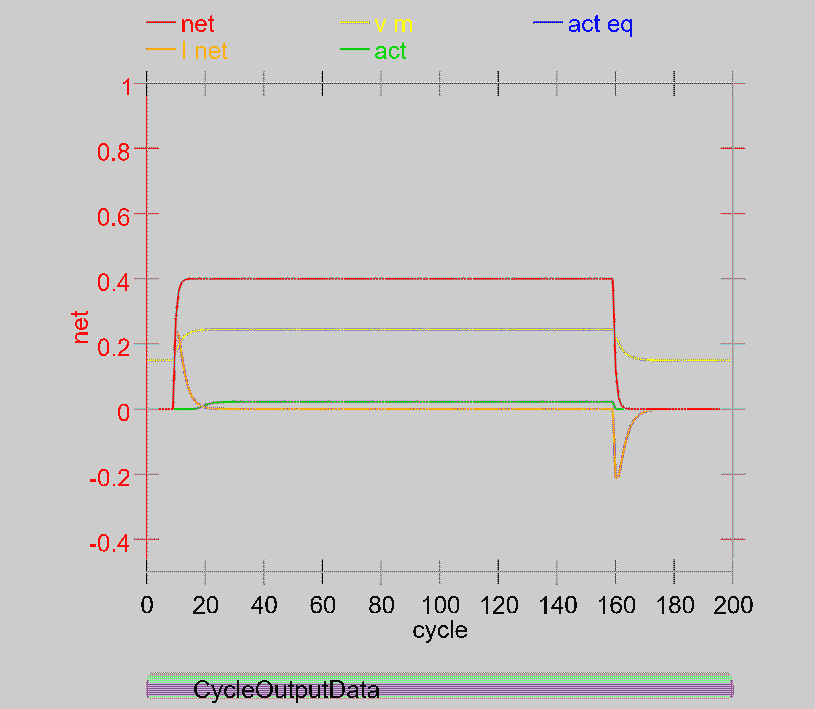
\includegraphics[scale=0.4]{Media/Main/EQ1/2.3.S2G.png}
\caption{Graphical output of the system where $g_{bar\_l}$ is at a value of 3.2.}
\label{Q2.32}
\end{figure}

\begin{figure}[H]
\centering
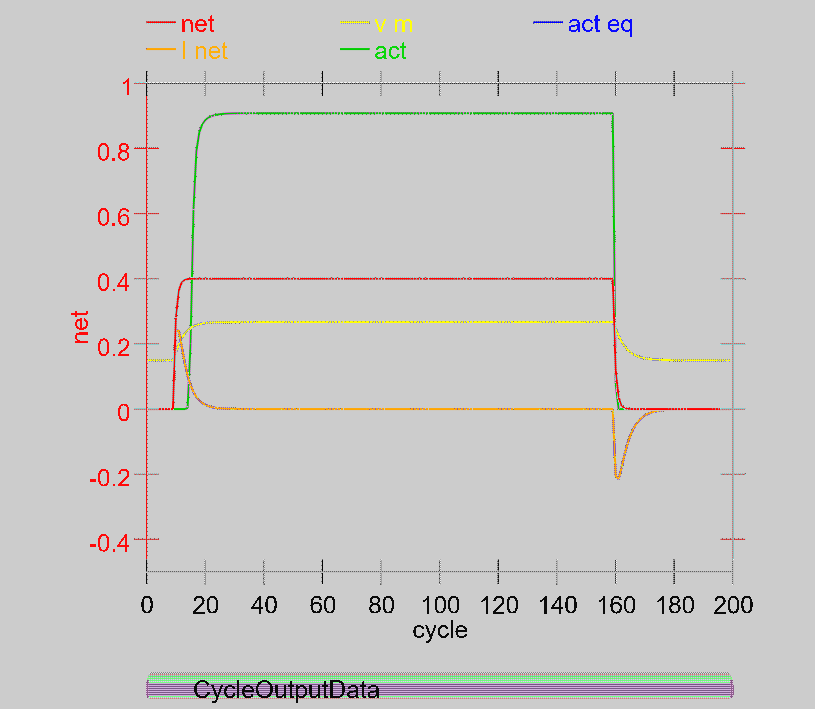
\includegraphics[scale=0.4]{Media/Main/EQ1/2.3.S3G.png}
\caption{Graphical output of the system where $g_{bar\_l}$ is at a value of 2.5.}
\label{Q2.33}
\end{figure}

\begin{figure}[H]
\centering
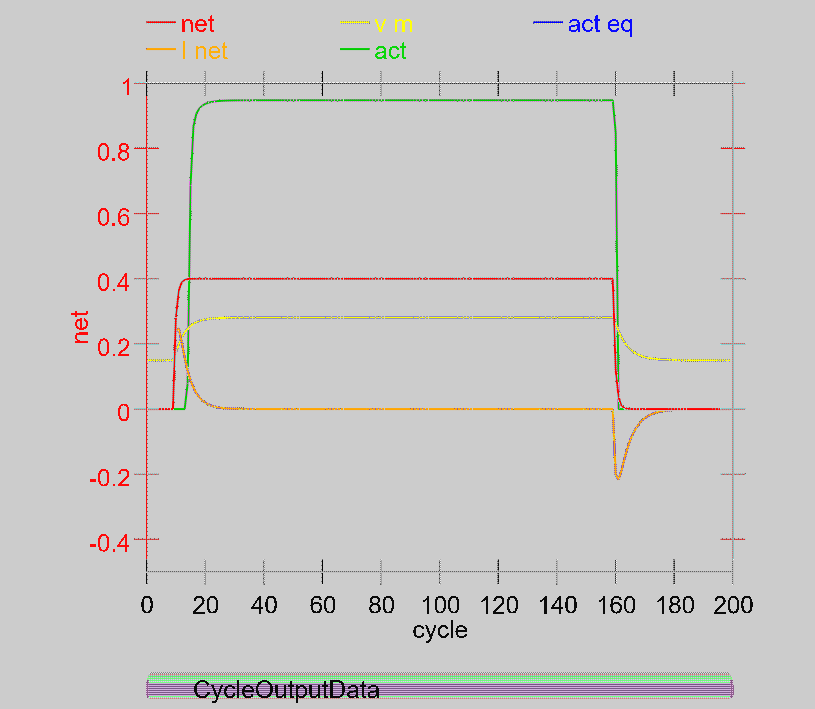
\includegraphics[scale=0.4]{Media/Main/EQ1/2.3.S4G.png}
\caption{Graphical output of the system where $g_{bar\_l}$ is at a value of 2.2.}
\label{Q2.34}
\end{figure}
\end{multicols}


\subsubsection{Task 2.4}
\label{Q1:Expl 2.6.1(2.4) SubSubSection}

\begin{tcolorbox}[colback=gray!20!white,colframe=gray!20!white]
  \emph{\textbf{Question 2.4 (a)} What happens to the unit’s activity if you change the leak reversal potential $e_{rev\_l}$ from .15 to 0? \textbf{(b)} What about when you increase it to .2? For both questions, explain the results, taking note of what happens before the input goes on as well as what happens while it is on. \textbf{(c)} What can you conclude about the relationship between the resting potential and the leak reversal potential? [Mark: 11]}
\end{tcolorbox} 
\vspace{0.5cm}

Changing the value of $e_{rev\_l}$ form 0.15 to 0 can be seen graphical in \cref{Q4.4} and \cref{Q4.5}. it can be seen when changing the leak reverse potential where the activation level equals to 0 and then when increasing it to 0.2 in \cref{Q4.6} the activation value reaches 1 in which influences the resulting membrane potential. When the $e_{rev\_l}$ is 0.2 the net current is identical to when $e_{rev\_l}$ is 0.15, this is probably due due to the small difference in value but can be seen with the rise of the activation value. However the net current starts negatives within the first 20 cycles (shown in \cref{Q4.5}) whereas when the value is positive the net current starts positive but both cases equal zero when the activation level is activated as the current is null while the activation level is reached. \\



\newpage
\begin{multicols}{2}
\begin{figure}[H]
\centering
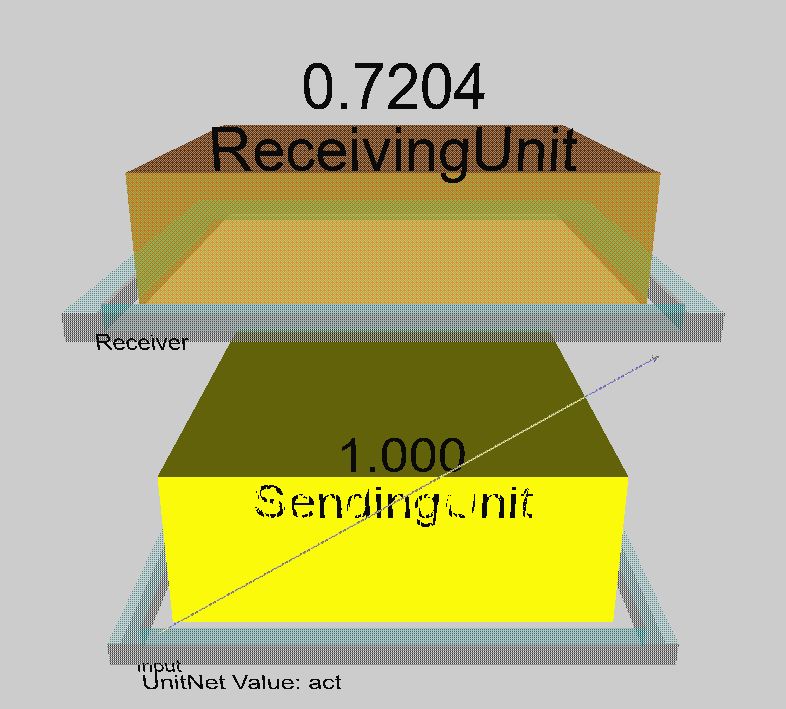
\includegraphics[scale=0.225]{Media/Main/EQ1/2.4.S0.png}
\caption{Visual representation of the sending and receiving units with $e_{rev\_l}$ at a value of 0.15.}
\label{Q4.1}
\end{figure}

\begin{figure}[H]
\centering
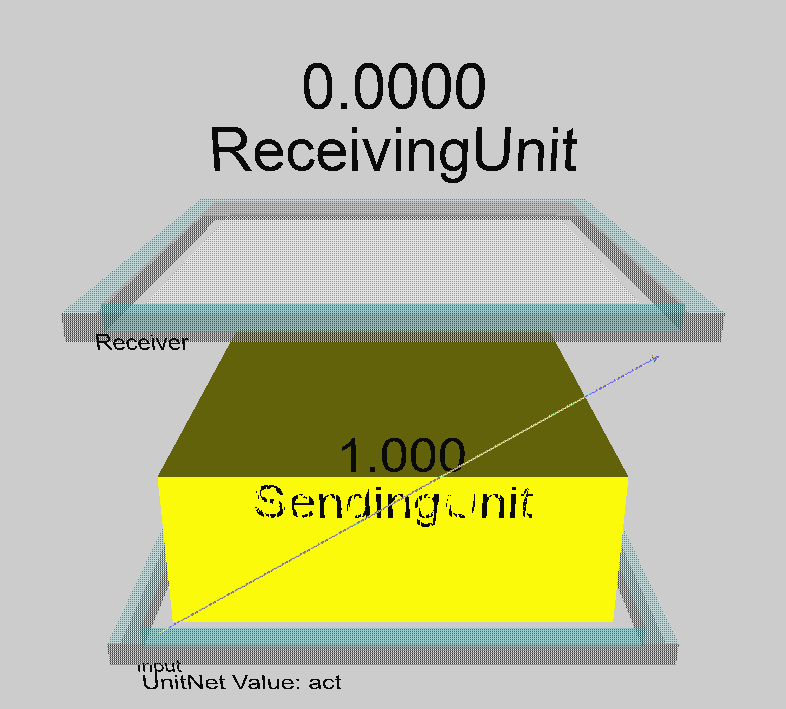
\includegraphics[scale=0.225]{Media/Main/EQ1/2.4.S1.png}
\caption{Visual representation of the sending and receiving units with $e_{rev\_l}$ at a value of 0.0.}
\label{Q4.2}
\end{figure}

\begin{figure}[H]
\centering
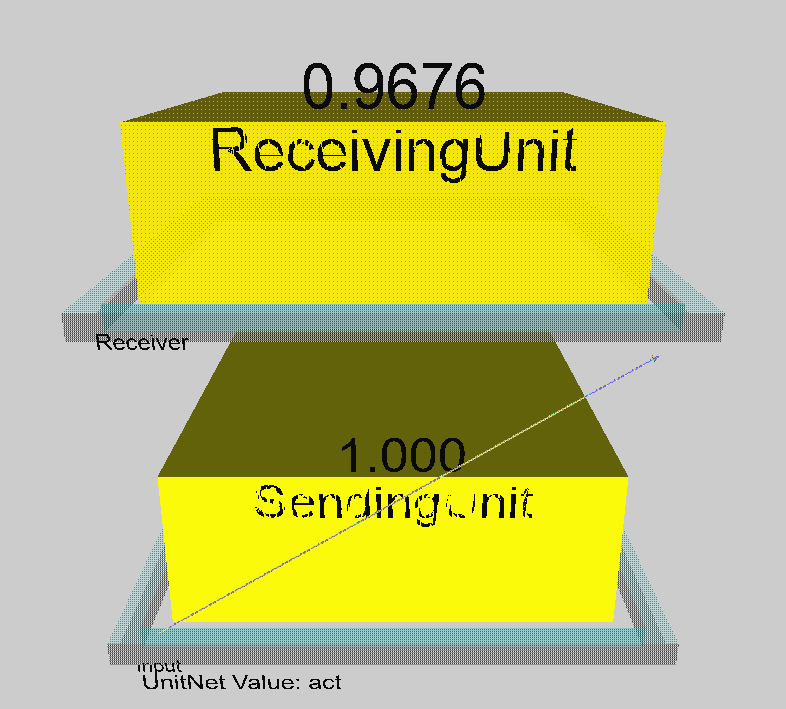
\includegraphics[scale=0.225]{Media/Main/EQ1/2.4.S2.png}
\caption{Visual representation of the sending and receiving units with $e_{rev\_l}$ at a value of 0.2.}
\label{Q4.3}
\end{figure}

\begin{figure}[H]
\centering
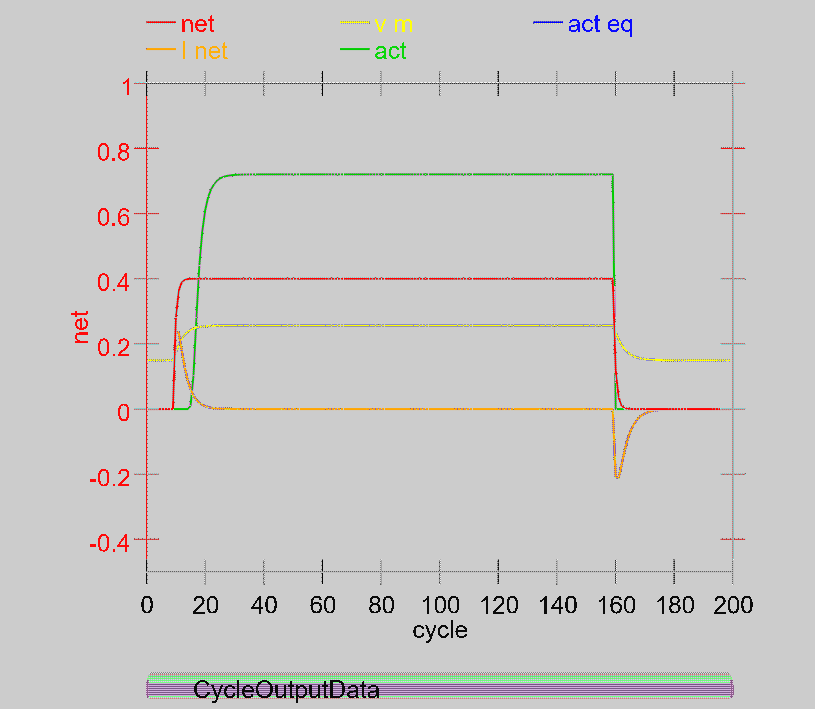
\includegraphics[scale=0.3]{Media/Main/EQ1/2.4.S0G.png}
\caption{Graphical output data of \cref{Q4.1} when running a value of 0.15 for $e_{rev\_l}$.}
\label{Q4.4}
\end{figure}

\begin{figure}[H]
\centering
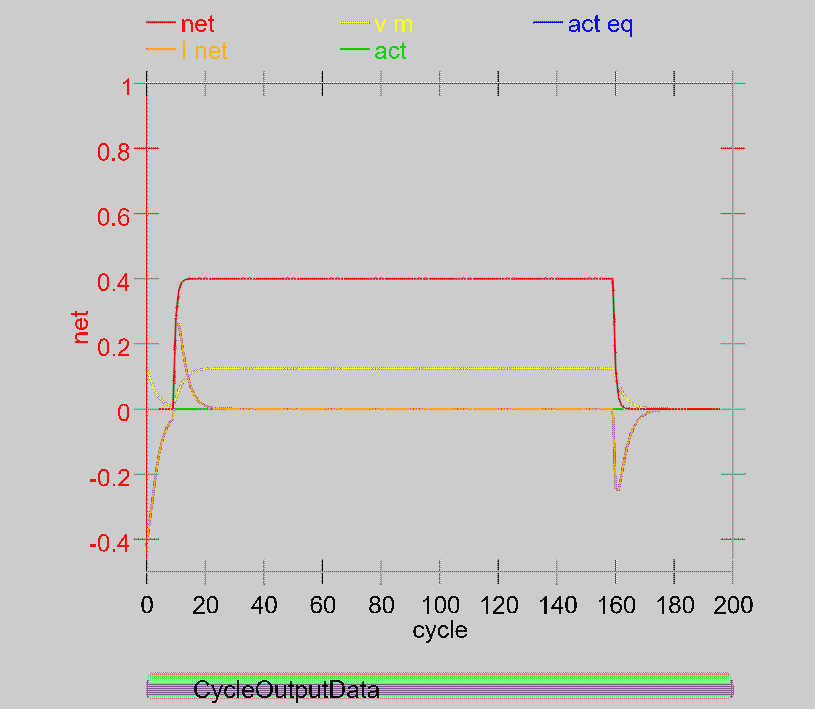
\includegraphics[scale=0.3]{Media/Main/EQ1/2.4.S1G.png}
\caption{Graphical output data of \cref{Q4.2} when running a value of 0.0 for $e_{rev\_l}$.}
\label{Q4.5}
\end{figure}

\begin{figure}[H]
\centering
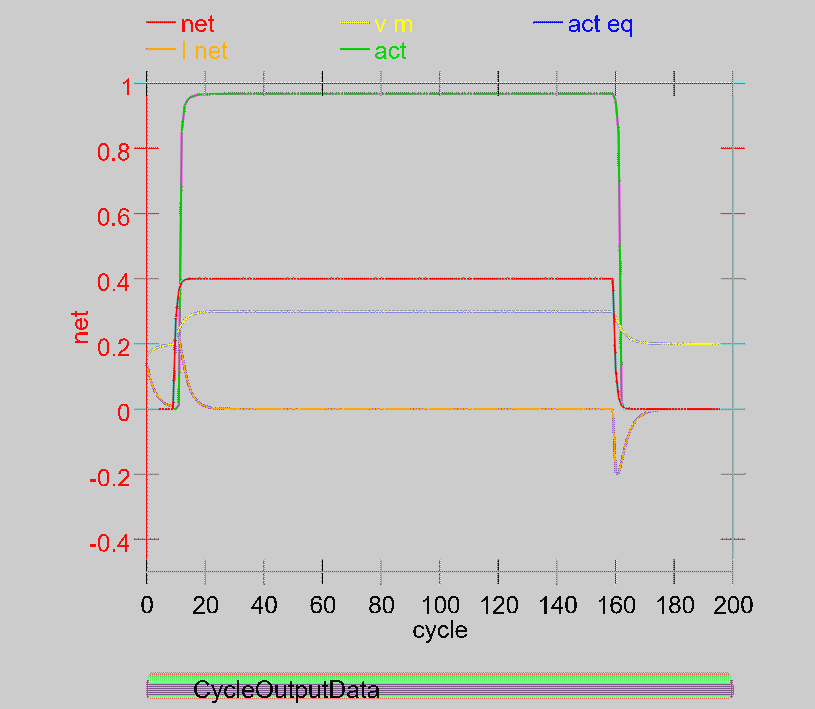
\includegraphics[scale=0.3]{Media/Main/EQ1/2.4.S2G.png}
\caption{Graphical output data of \cref{Q4.3} when running a value of 0.2 for $e_{rev\_l}$.}
\label{Q4.6}
\end{figure}
\end{multicols}

\subsubsection{Task 2.5}
\label{Q1:Expl 2.6.1(2.5) SubSubSection}

\begin{tcolorbox}[colback=gray!20!white,colframe=gray!20!white]
  \emph{\textbf{Question 2.5 (a)} What happens to the unit’s activity if you change the excitatory reversal potential $e_{rev\_e}$ from 1 to .5? Why does this happen? \textbf{(b)} Can you com- pensate for this by changing the value of $g_{bar\_e}$? To two decimal places, use the simulator to find the value of $g_{bar\_e}$ that gives essentially the same activation value as the default parameters. \textbf{(c)} Then use the same approach as in question 2.2 to solve for the exact value of $g_{bar\_e}$ that will compensate for this change in $e_{rev\_e}$ (use .256 for the membrane potential under the default parameters, and show your math). [Mark: 10]}
\end{tcolorbox} 
\vspace{0.5cm}

By changing the excitatory reversal potential $e_{rev\_e}$ value from 1.0 to 0.5 as seen in \cref{Q5.4}, the activation value is zero this is because the excitatory reversal potential must equal to 1 for any response in the activation level as the $g_{bar\_e}$ is at 0.4. The defaults parameters gave an activation level of 0.204, in \cref{Q5.5} where the value of $g_{bar\_e}$ is 1.22 which gives an activation level of 0.7191, this is the closest to the activation level to two decimal places. \\

\newpage
\begin{multicols}{2}
\begin{figure}[H]
\centering
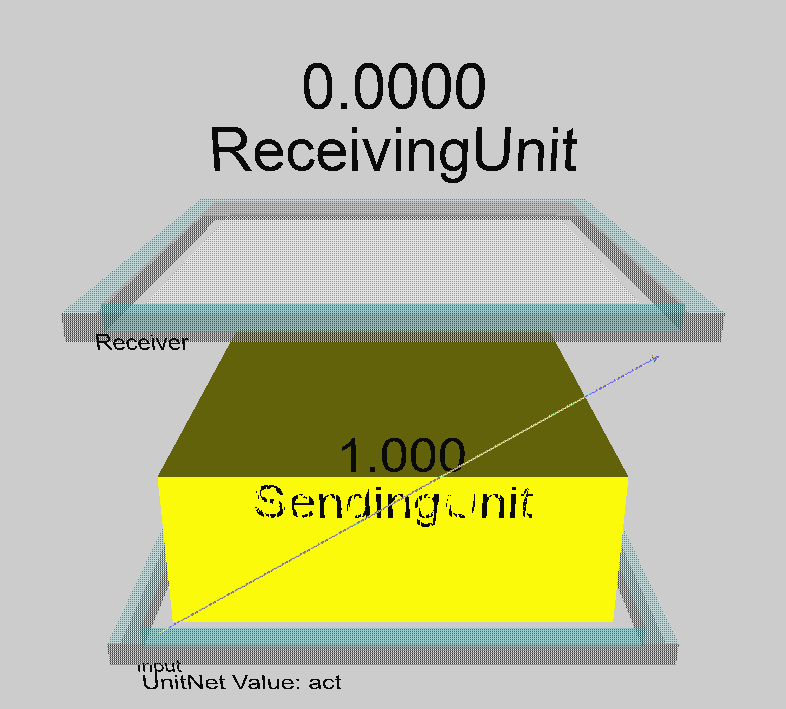
\includegraphics[scale=0.225]{Media/Main/EQ1/2.5.S1.png}
\caption{Visual representation of the sending and receiving units with $g_{rev\_e}$ at a value of 0.4.}
\label{Q5.1}
\end{figure}

\begin{figure}[H]
\centering
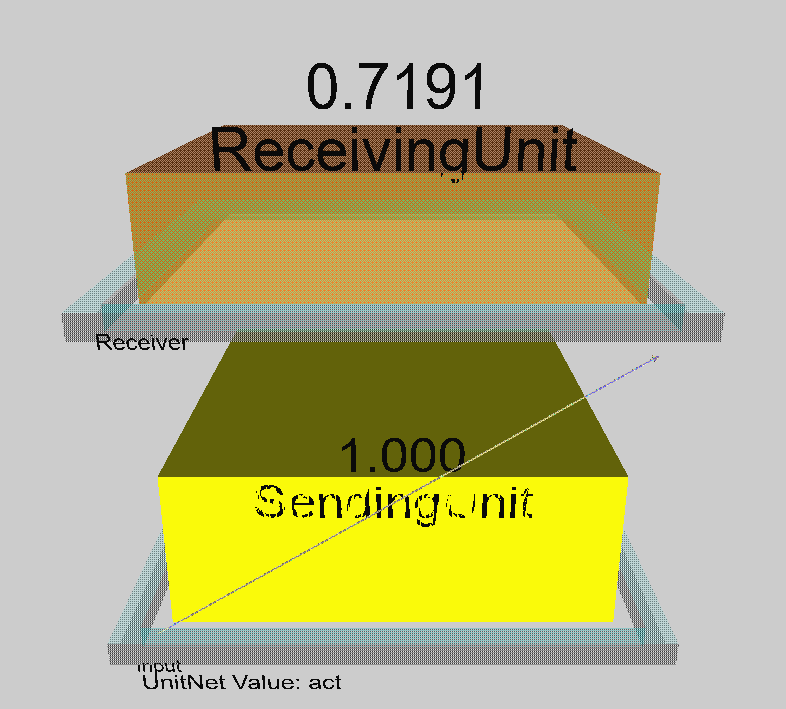
\includegraphics[scale=0.225]{Media/Main/EQ1/2.5.S2.png}
\caption{Visual representation of the sending and receiving units with $g_{rev\_e}$ at a value of 1.22.}
\label{Q5.2}
\end{figure}

\begin{figure}[H]
\centering
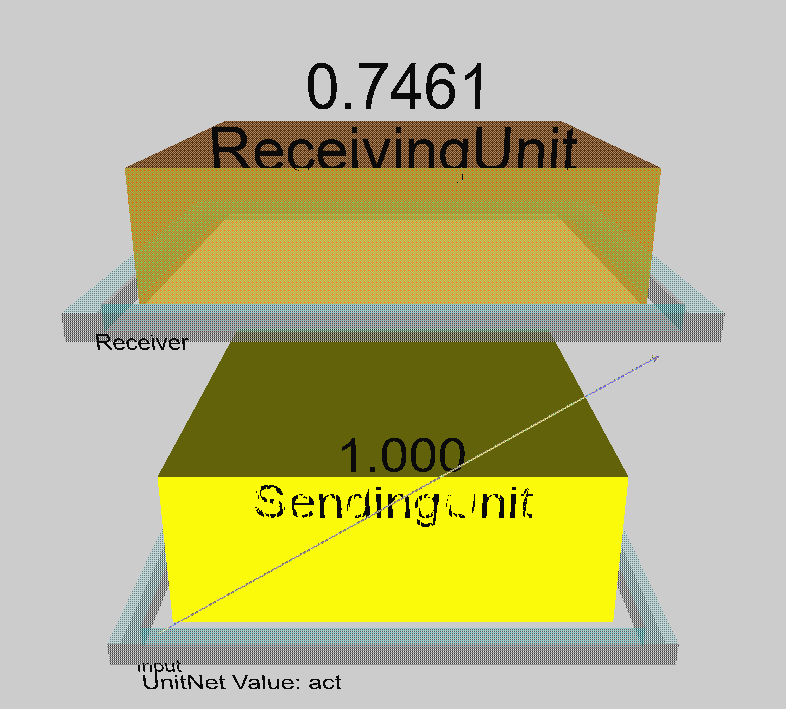
\includegraphics[scale=0.225]{Media/Main/EQ1/2.5.S3.png}
\caption{Visual representation of the sending and receiving units with $g_{rev\_e}$ at a value of 1.23.}
\label{Q5.3}
\end{figure}

\begin{figure}[H]
\centering
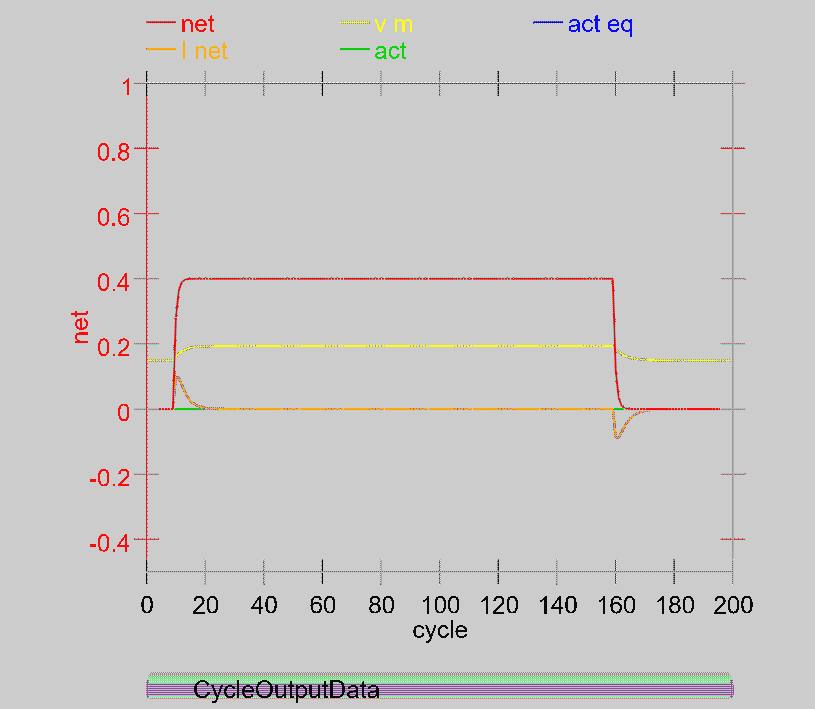
\includegraphics[scale=0.3]{Media/Main/EQ1/2.5.S1G.png}
\caption{Graphical output data of \cref{Q5.1} when running a value of 0.4 for $g_{rev\_e}$.}
\label{Q5.4}
\end{figure}

\begin{figure}[H]
\centering
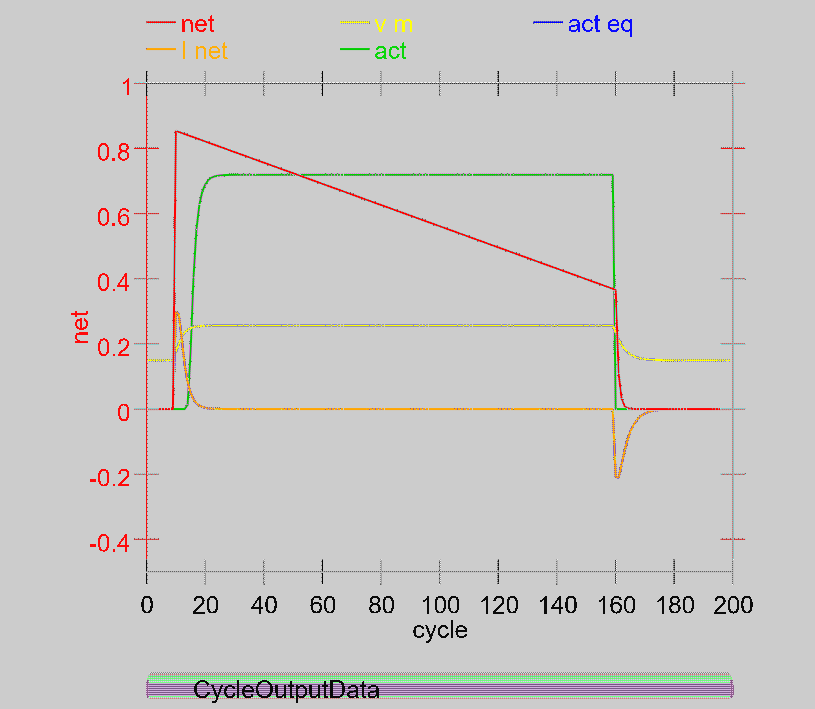
\includegraphics[scale=0.3]{Media/Main/EQ1/2.5.S2G.png}
\caption{Graphical output data of \cref{Q5.2} when running a value of 1.22 for $g_{rev\_e}$.}
\label{Q5.5}
\end{figure}

\begin{figure}[H]
\centering
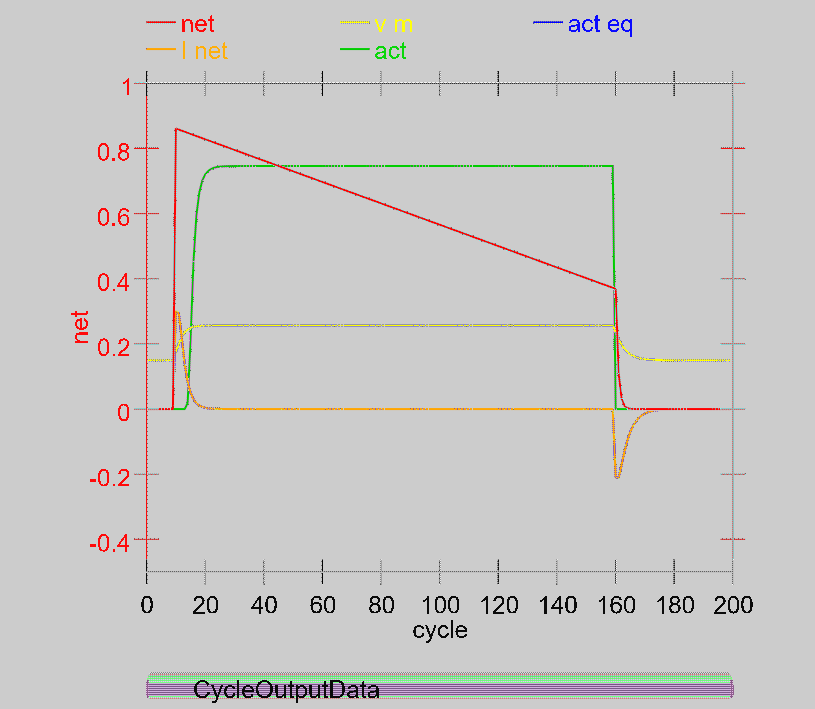
\includegraphics[scale=0.3]{Media/Main/EQ1/2.5.S3G.png}
\caption{Graphical output data of \cref{Q5.3} when running a value of 1.23 for $g_{rev\_e}$.}
\label{Q5.6}
\end{figure}
\end{multicols}
\subsection{Q2: Exploration 2.6.3 (Page 55)}
\label{Q2:Expl 2.6.3 SubSection}

\subsubsection{Task 2.7}
\label{Q1:Expl 2.6.3(2.7) SubSubSection}

\begin{tcolorbox}[colback=gray!20!white,colframe=gray!20!white]
  \emph{\textbf{Question 2.7 (a)} For each digit, report the number of input units where there is a weight of 1 and the input unit is also active. This should be easily visually perceptible in the display. You should find some variability in these numbers across the digits. \textbf{(b)} Why does the activation value of the receiving unit not reflect any of this variability? \textbf{(c)} What would be a better variable to examine in order to view this underlying variability, and why? [Mark: 10]}
\end{tcolorbox} 
\vspace{0.5cm}

In \cref{Q2.7A-Connected Digits} is the tabulated data record from the Emergent software. The data presented is the input data that is given to the receiving unit in the form of input patterns that display as digits from 0 to 9. In each individual digit, there are specific input data that activate it as seen in \cref{Q2.7.1} by the yellow (lit) up squares, these connect and directly relate to the receiving unit as depicted by the yellow lines. \\

The reason behind the receiving unit only activating on the number 8 digit in because all 17 input points are connected to the receiving unit whereas for the other 9 digits only up to 80\% of them are connected where the weights are easily distinguishable in \cref{Q2.7.1}. A better value to examine would be the net values of $e_{bar\_l}$ as it alters the activation value of each input unit without changing the original excitatory conductance ($e_{bar\_e}$).

\begin{table}[H]
\begin{center}
 \footnotesize
 \begin{tabular}{|c||c|c|c|}
 \hline
 \multicolumn{4}{|c|}{Number of connected and active inputs for each individual digit.} \\
 \hline \hline
 Digits & Connected& Active& Value of\\
  & (Weight of 1) & (Active Sensors)& Receiving Unit\\
 \hline \hline
 0 & 6 & 12 & 0.0000 \\\hline
 1 & 6 & 13 & 0.0000 \\\hline
 2 & 12 & 15 & 0.0000 \\\hline
 3 & 13 & 15 & 0.0000 \\\hline
 4 & 5 & 14 & 0.0000 \\\hline
 5 & 14 & 16 & 0.0000 \\\hline
 6 & 12& 15 & 0.0000 \\\hline
 7 & 6 & 11 & 0.0000 \\\hline
 8 & 17 & 17 & 0.9500 \\\hline
 9 & 12 & 15 & 0.0000 \\\hline
 \end{tabular} \\ 
 \caption{Number of connected and active inputs for each individual digit.}
 \label{Q2.7A-Connected Digits}
\end{center}
\end{table}

\begin{figure}[H]
\centering
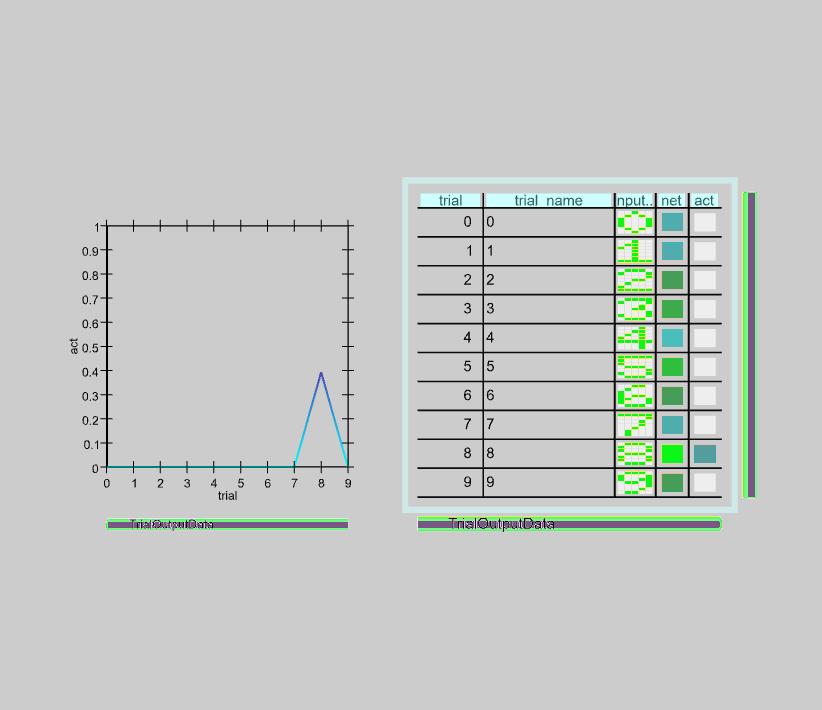
\includegraphics[scale=0.5]{Media/Main/EQ2/2.7-S0.png}
\caption{Graphical output of a full run cycle for this project.}
\label{Q2.7.0}
\end{figure}

\begin{figure}[H]
\centering
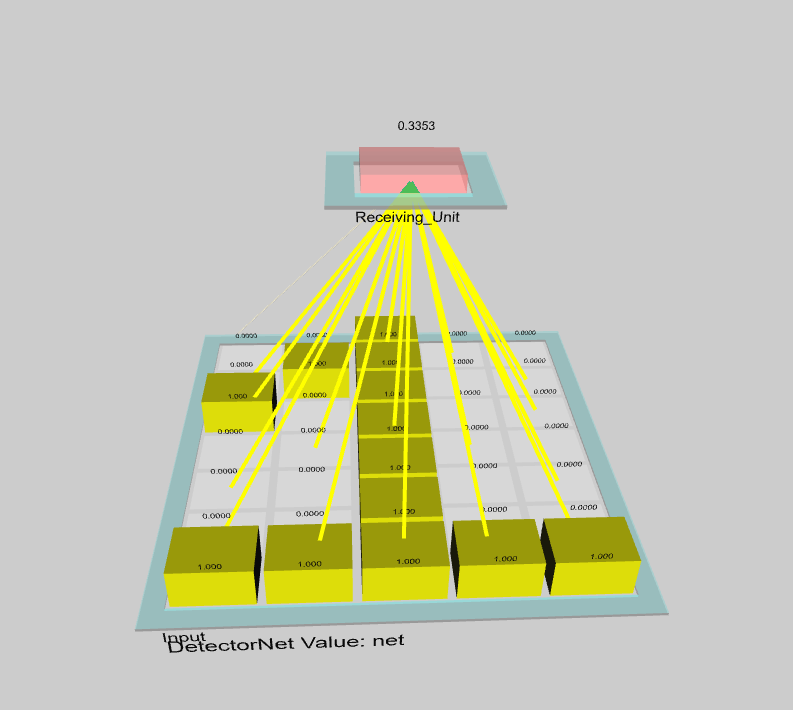
\includegraphics[scale=0.5]{Media/Main/EQ2/2.7-S1.png}
\caption{Visual representation of the connected data, input data and receiving unit.}
\label{Q2.7.1}
\end{figure}

\subsubsection{Task 2.9}
\label{Q1:Expl 2.6.3(2.9) SubSubSection}

\begin{tcolorbox}[colback=gray!20!white,colframe=gray!20!white]
  \emph{\textbf{Question 2.9 (a)} What happens to the pattern of receiving unit activity when you reduce $g_{bar\_l}$ to 6? \textbf{(b)} What happens with $g_{bar\_l}$ values of 4, 1, and 8? \textbf{(c)} Explain the effect of changing $g_{bar\_l}$ in terms of the point neuron activation function. \textbf{(d)} What might the consequences of these different response patterns have for other units that might be listening to the output of this receiving unit? Try to give some possible advantages and disadvantages for both higher and lower values of $g_{bar\_l}$. [Mark: 13]}
\end{tcolorbox} 
\vspace{0.5cm}

The default settings for the value of $g_{bar\_l}$ is 7, decreasing it to a value of 6 increases the activation value on the number 8 digit from 0.3930 to 0.9024. Changing the values of $g_{bar\_l}$ to 4, 1 and 8 are shown in \cref{Q2.9 Table} for all the digits show a direct relationship between $g_{bar\_l}$ and the receiving unit. By changing the $g_{bar\_l}$, the point neuron activation function changes in terms of the threshold and the change in $g_{bar\_l}$ changes the threshold allowing for the change in activation value. It's seen that as $g_{bar\_l}$ is decreased the activation value increases in the receiving unit and observing the value change in \cref{Q2.9 Table} and it can also been seen that the lower values of $g_{bar\_l}$ allows for the surrounding units to copy in weight and as such allows the digits to activate the receiving unit. The higher the number the more accurate the weight is and therefore the number 8 digit is the only one that can activate the receiving unit so therefore the higher the value of $g_{bar\_l}$ the more accurate the weights of the individual units.

\begin{table}[H]
\begin{center}
 \footnotesize
 \begin{tabular}{|c||c|c|c|c|c|c|c|c|c|c|}
 \hline
 \multicolumn{11}{|c|} {} \\
 $g_{bar\_l}$ & No. 0 & No.1 & No.2 & No.3 & No.4 & No.5 & No.6 & No.7 & No.8 & No.9 \\ 
 \hline \hline
 7 & 0 & 0 & 0 & 0 & 0 & 0 & 0 & 0 & 8.3930 & 0 \\\hline
 6 & 0 & 0 & 0.0033 & 0 & 0.1357 & 0 & 0 & 0 & 0.9024 & 0\\\hline
 4 & 0 & 0 & 0.9280 & 0.9478 & 0 & 0.9588 & 0.9280 & 0 & 0.9742 & 0.9280 \\\hline
 1 & 0.9842 & 0.9842 & 0.9925 & 0.9929 & 0.9788 & 0.9932 & 0.9925 & 0.9842 & 0.9938 & 0.9925 \\\hline
 8 & 0 & 0 & 0 & 0 & 0 & 0 & 0 & 0 & 0.0009 & 0 \\\hline
 \end{tabular} \\ 
 \caption{Recieving values for individual digits with different $g_{bar\_l}$ values.}
 \label{Q2.9 Table}
\end{center}
\end{table}
\subsection{Q3: Exploration 3.4.2 (Page 87)}
\label{Q3:Expl 3.4.2 SubSection}

\subsubsection{Task 3.7}
\label{Q1:Expl 3.4.2 (3.7) SubSubSection}

\begin{tcolorbox}[colback=gray!20!white,colframe=gray!20!white]
  \emph{\textbf{Question 3.7 (a)} Given the pattern of weights, what is the minimal number of units that need to be clamped to produce pattern completion to the full 8? You can determine your answer by toggling off the units in the event pattern one-by-one until the network no longer produces the complete pattern when it is Run (don’t forget to press Apply in the environment window after clicking).\textbf{(b)} The $g_{bar\_l}$ parameter can be altered to lower this minimal number. What value of this parameter allows completion with only one input active? [Mark: 6]} 
\end{tcolorbox} 
\vspace{0.5cm}

With 17 units turned on, the pattern is a visible whereas when 18 units are active the the number 8 is not display at full, this is because due to only 17 units being connected to the receiving unit. $g_{bar\_l}$ can be changed from a value of 7 to 3 to which only one input is active.

\begin{figure}[H]
\centering
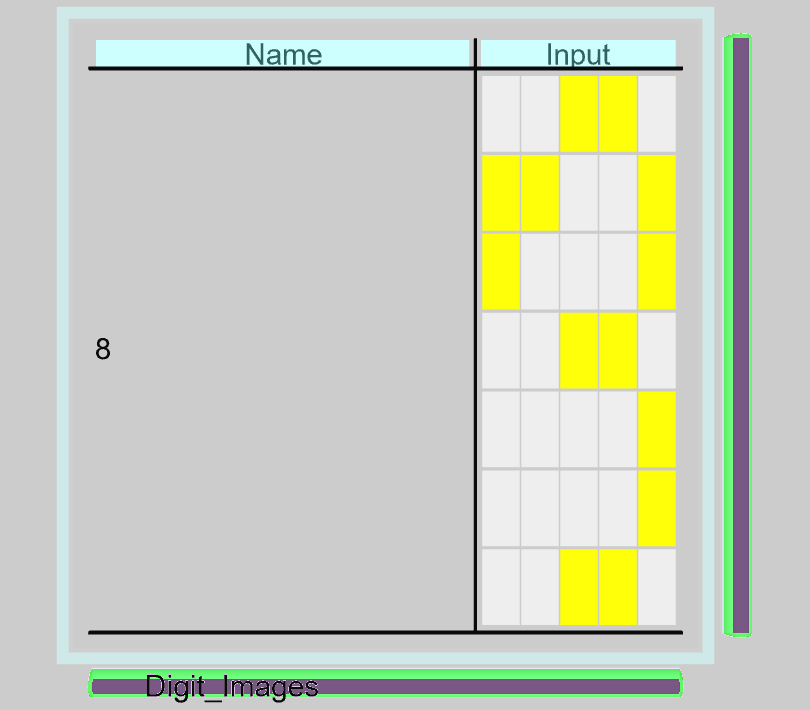
\includegraphics[scale=0.5]{Media/Main/EQ3/S0.png}
\caption{.}
\label{Q3.2}
\end{figure}

\subsubsection{Task 3.8}
\label{Q1:Expl 3.4.2 (3.8) SubSubSection}

\begin{tcolorbox}[colback=gray!20!white,colframe=gray!20!white]
  \emph{\textbf{Question 3.8 (a)} What happens if you activate only inputs which are not part of the 8 pattern? Why? \textbf{(b)} Could the weights in this layer be configured to support the representation of another pattern in addition to the 8 (such that this new pattern could be distinctly activated by a partial input), and do you think it would make a difference how similar this new pattern was to the 8 pattern? Explain your answer. [Mark: 7]} 
\end{tcolorbox} 
\vspace{0.5cm}

When inputs are activated that aren't part of the number 8 digits pattern the image disappears because the weight values of the unit is equal 0. The new pattern could be the number 3 digits as shown in \cref{Q3.2} as enough input units are activated to produce the number 3 digit pattern as it uses the same pattern units as the number 8 digit minus a few units.

\section{Further Questions}
\label{Further Questions Section}
\subsection{Further Question 1}
\label{Further Question 1 SubSection}

\begin{tcolorbox}[colback=gray!20!white,colframe=gray!20!white]
  \emph{Why are the O’Reilly and Munakata equations called point neuron equations? As a consequence of this, what aspects of neurophysiology can these equations not reflect?[Mark: 6]}
\end{tcolorbox} 
\vspace{0.5cm}


\subsection{Further Question 2}
\label{Further Question 2 SubSection}

\begin{tcolorbox}[colback=gray!20!white,colframe=gray!20!white]
  \emph{In the output activation equation below, what would the consequence be of replacing the +1 term with +10? How could one obtain a similar effect by changing a parameter of this equation? [Mark: 7]}

\begin{equation}
    y_j = \frac{\gamma[V_m - \Theta]_+}{\gamma[V_m - \Theta]_+ + 1}
\end{equation}
\end{tcolorbox} 
\vspace{0.5cm}

By plotting the rate code output function above and using $V_m$ as the unknown variable where $\gamma$ and $\Theta$ are fixed variables, it's seen that by increasing the denominator from +1 to +10, the output activation value ($y_j$) decreases in value as when compared to +1. 

%\newpage
%\bibliographystyle{plain}
%\bibliography{mybib}

%\newpage
%\section{Appendix}
%\label{Appendix Section}
%\subsection{Magnox Mini Project Plan}
\label{Project Plan SubSection}

\subsubsection*{Project Outline:}
\label{Project Outline SubSubSection}

With nuclear waste within the UK on the rise, more nuclear waste is being made as the projection of power that is made by nuclear power plants is likely to increase in the next decade. The goal of this mini project in relation to Magnox nuclear waste is to design a cheap, strong, reliable and feasible container that will hold and transport nuclear waste. I will begin researching the type of nuclear waste the UK disposes of and how its currently transported and disposed of, then I will look at specific materials used to transport nuclear waste, why they are used and highlight positives and negatives of these methods. From this research I will begin designing and constructing the ideal container factoring in variables such as the intensity of radioactive waste against the type and size of the materials used in the container and what happens to the containers after transporting radioactive waste. By researching what radioactive waste is being disposed of and how it will get to the specified facility, I can specify what hazards the container may face without cracking, leaking or breaking the inner core that holds the radioactive waste. \\

As I cannot physically build and test such a container, I will gather data from scientific journals to show the penetration of gamma rays, x-rays, alpha and beta particles through lead. Through these values and my understanding of nuclear and particle physics I shall calculate numerous values for the tensile strength, weight, ray penetration (leakage), material degradation and other key factors. Ultimately, I shall have to prove mathematically that the container works. \\

My current theoretical proposal is a hexagonal container lined with lead core surrounded by a perpendicular titanium honeycomb inner wall, covered by aluminium or another composite material. Its proven that the thickness and quality of the lead wall greatly determines the penetration of gamma rays, which ultimately will affect the design of the container. The container should be as light weight as possible without prompting any hazards, the proposed titanium honeycomb wall shall improve the strength of the container and prevent deformation of the lead core and the aluminium / composite material will act protect the honeycomb structure from wear and tear, rust and other environmental hazards allowing the container to be built to last. 

\subsubsection*{Magnox Nuclear Waste Project Timeline:}
\label{Magnox Nuclear Waste Project Timeline SubSubSection}
\vspace{0.2cm}

\textbf{\underline{Week 10:}} \\ [0.2cm]
Initial mini project option selected. The construction of this project plan will act as a guide for this project and give weekly goals to achieve.\\ 

\textbf{\underline{Week 11:}} \\ [0.2cm]
Basic research completed, construct multiple ideas for a container to work off of. The submission and finalisation of the project plan. The project report to be started and the project report introduction to be wrote.\\

\textbf{\underline{Week 12:}} \\ [0.2cm]
Start research relating to the restrictions of the container such as materials, shapes, general design and thus a series of crude ideas and possible designs to be constructed. Thus, start the research in section the project report.\\

\textbf{\underline{Week 13:}} \\ [0.2cm]
Finish all research and start looking at a series of ideal materials for the construction of the container, calculations of the containment of radioactive material through gamma ray, x-ray, alpha and beta particles penetration of the material will be used to prove the most ideal material.\\

\textbf{\underline{Week 14:}} \\ [0.2cm]
Finish all research. Start finalising 2/3 designs and proving all positives and negatives and compare them. Proving through mathematical calculations of radioactive penetration and strength will be used to primarily judge which design is the best to pursue.\\

\textbf{\underline{Week 15:}} \\ [0.2cm]
Complete all current sections in the project report (Introduction, research, designs). Continues with calculation proving that the chosen design work and is suitable for the task its design to do and hazards it will face. Investigate errors and develop a report of these errors and ensure these errors are within suitable parameters (previously researched).\\

\textbf{\underline{Week 16:}} \\ [0.2cm]
Finish all calculations and finalise the design of the container allowing for the error analysis, complete the final design section in the project report include final calculations, schematics and errors.\\

\textbf{\underline{Week 17:}} \\ [0.2cm]
This week is allocated to allow as a buffer week in case of any problems encountered throughout the project. If not, problems are encounter then it shall be used as a pre-finalisation of my final report and check of error analysis.\\

\textbf{\underline{Week 18:}} \\ [0.2cm]
Finalise and check all research, calculations, errors, designs and report. Produce project analysis and conclusion. Submit project report.\\


%--------------------------------------------------------------------------------
\end{document}